\documentclass[a4paper]{article}

\usepackage[margin=1.5cm]{geometry}  % tweak margins as you like
\usepackage{graphicx}
\usepackage{subcaption}              % only for arranging panels (no sub-captions used)
\pagestyle{empty}
%\usepackage[numbers]{natbib}
%\usepackage[authoryear]{natbib}
\usepackage[numbers]{natbib}
%% The amssymb package provides various useful mathematical symbols
\usepackage{amssymb}
%% The amsmath package provides various useful equation environments.
\usepackage{amsmath}
\usepackage{epstopdf}
\usepackage{mathptmx,mathtools}
\usepackage{subcaption}
\usepackage{float} % Add this in your preamble
\usepackage[export]{adjustbox}
\usepackage{array} % Needed for m{} column type


\usepackage{amsmath}
\usepackage{nicefrac}
\usepackage{dirtytalk}
\usepackage{graphicx}   % For including images
\usepackage{tikz}       % For drawing arrows
\usepackage{xcolor}     % For coloring
\usepackage{lineno}
\renewcommand\linenumberfont{\normalfont\bfseries\small} % <-- Increase line number size

\begin{document}

	\begin{figure}[!tbp]
	\centering
	
	% Row 1: (a) and (b)
	\begin{subfigure}[t]{0.49\textwidth}
		\centering
		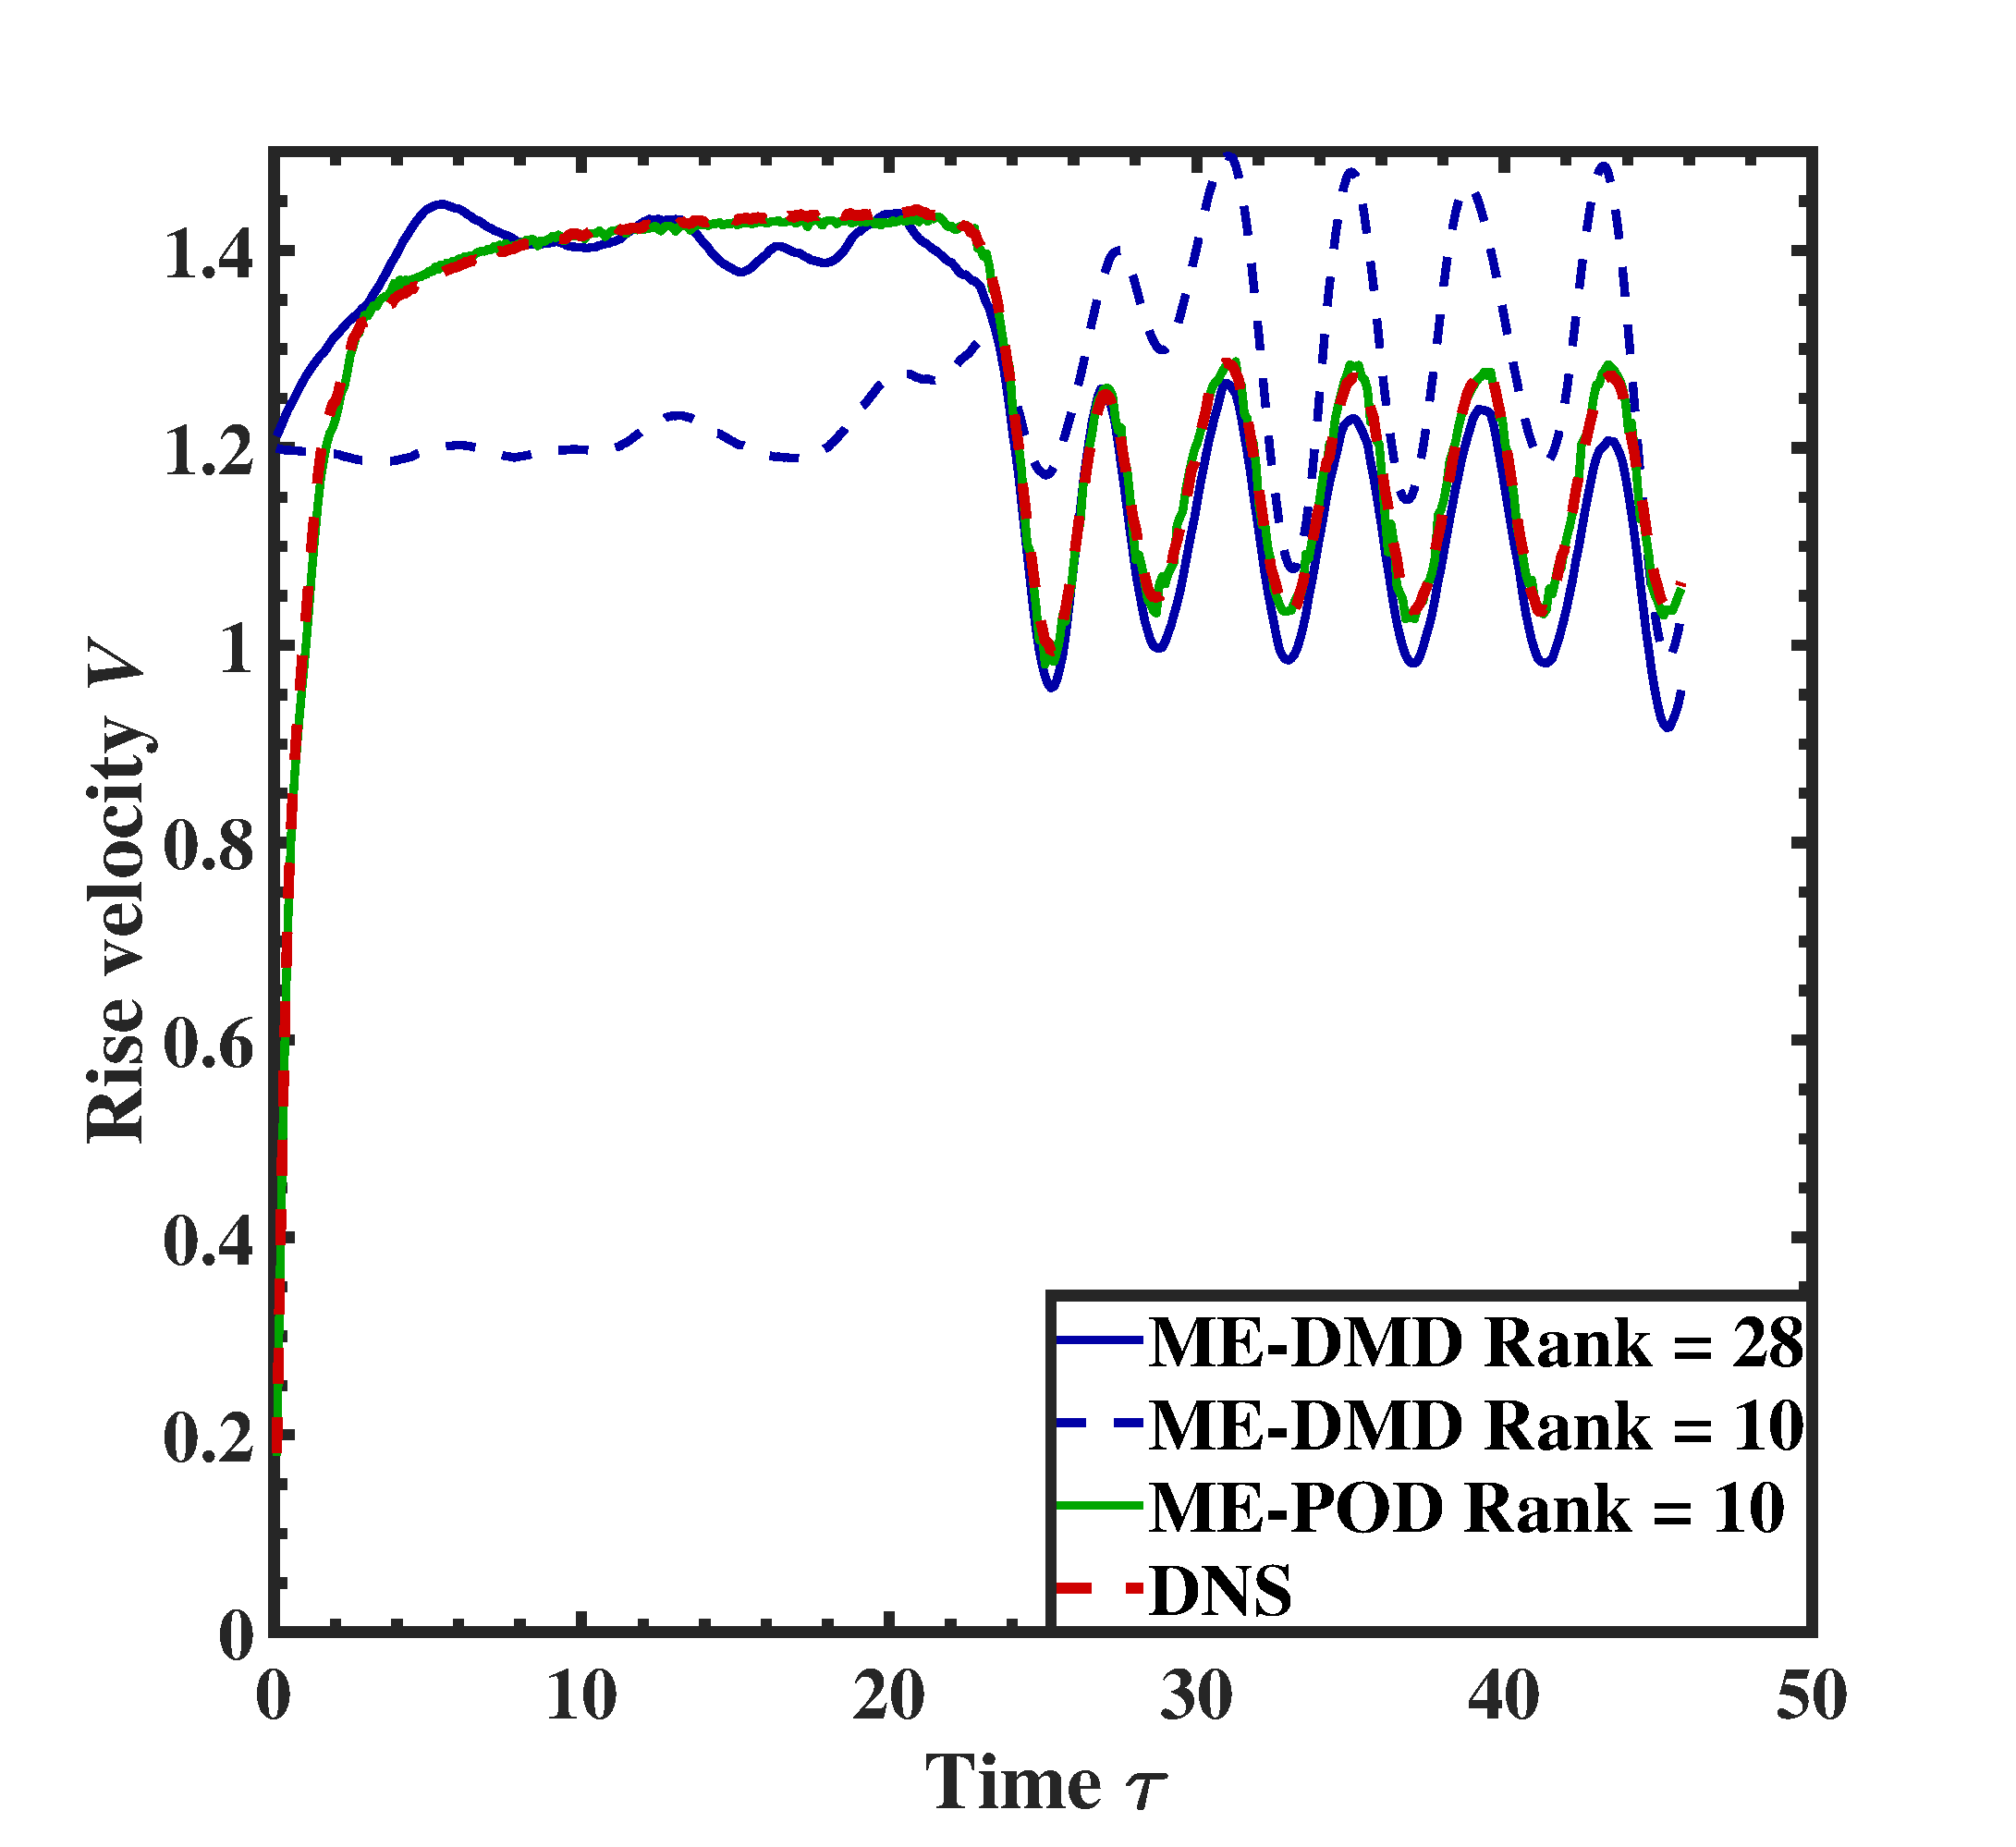
\includegraphics[scale=0.24,trim={0.5cm 0.3cm 2.5cm 2cm},clip]{Figure7a.eps}
		\put(-215,219){\large\textbf{(a)}}
	\end{subfigure}
	\hfill
	\begin{subfigure}[t]{0.49\textwidth}
		\centering
		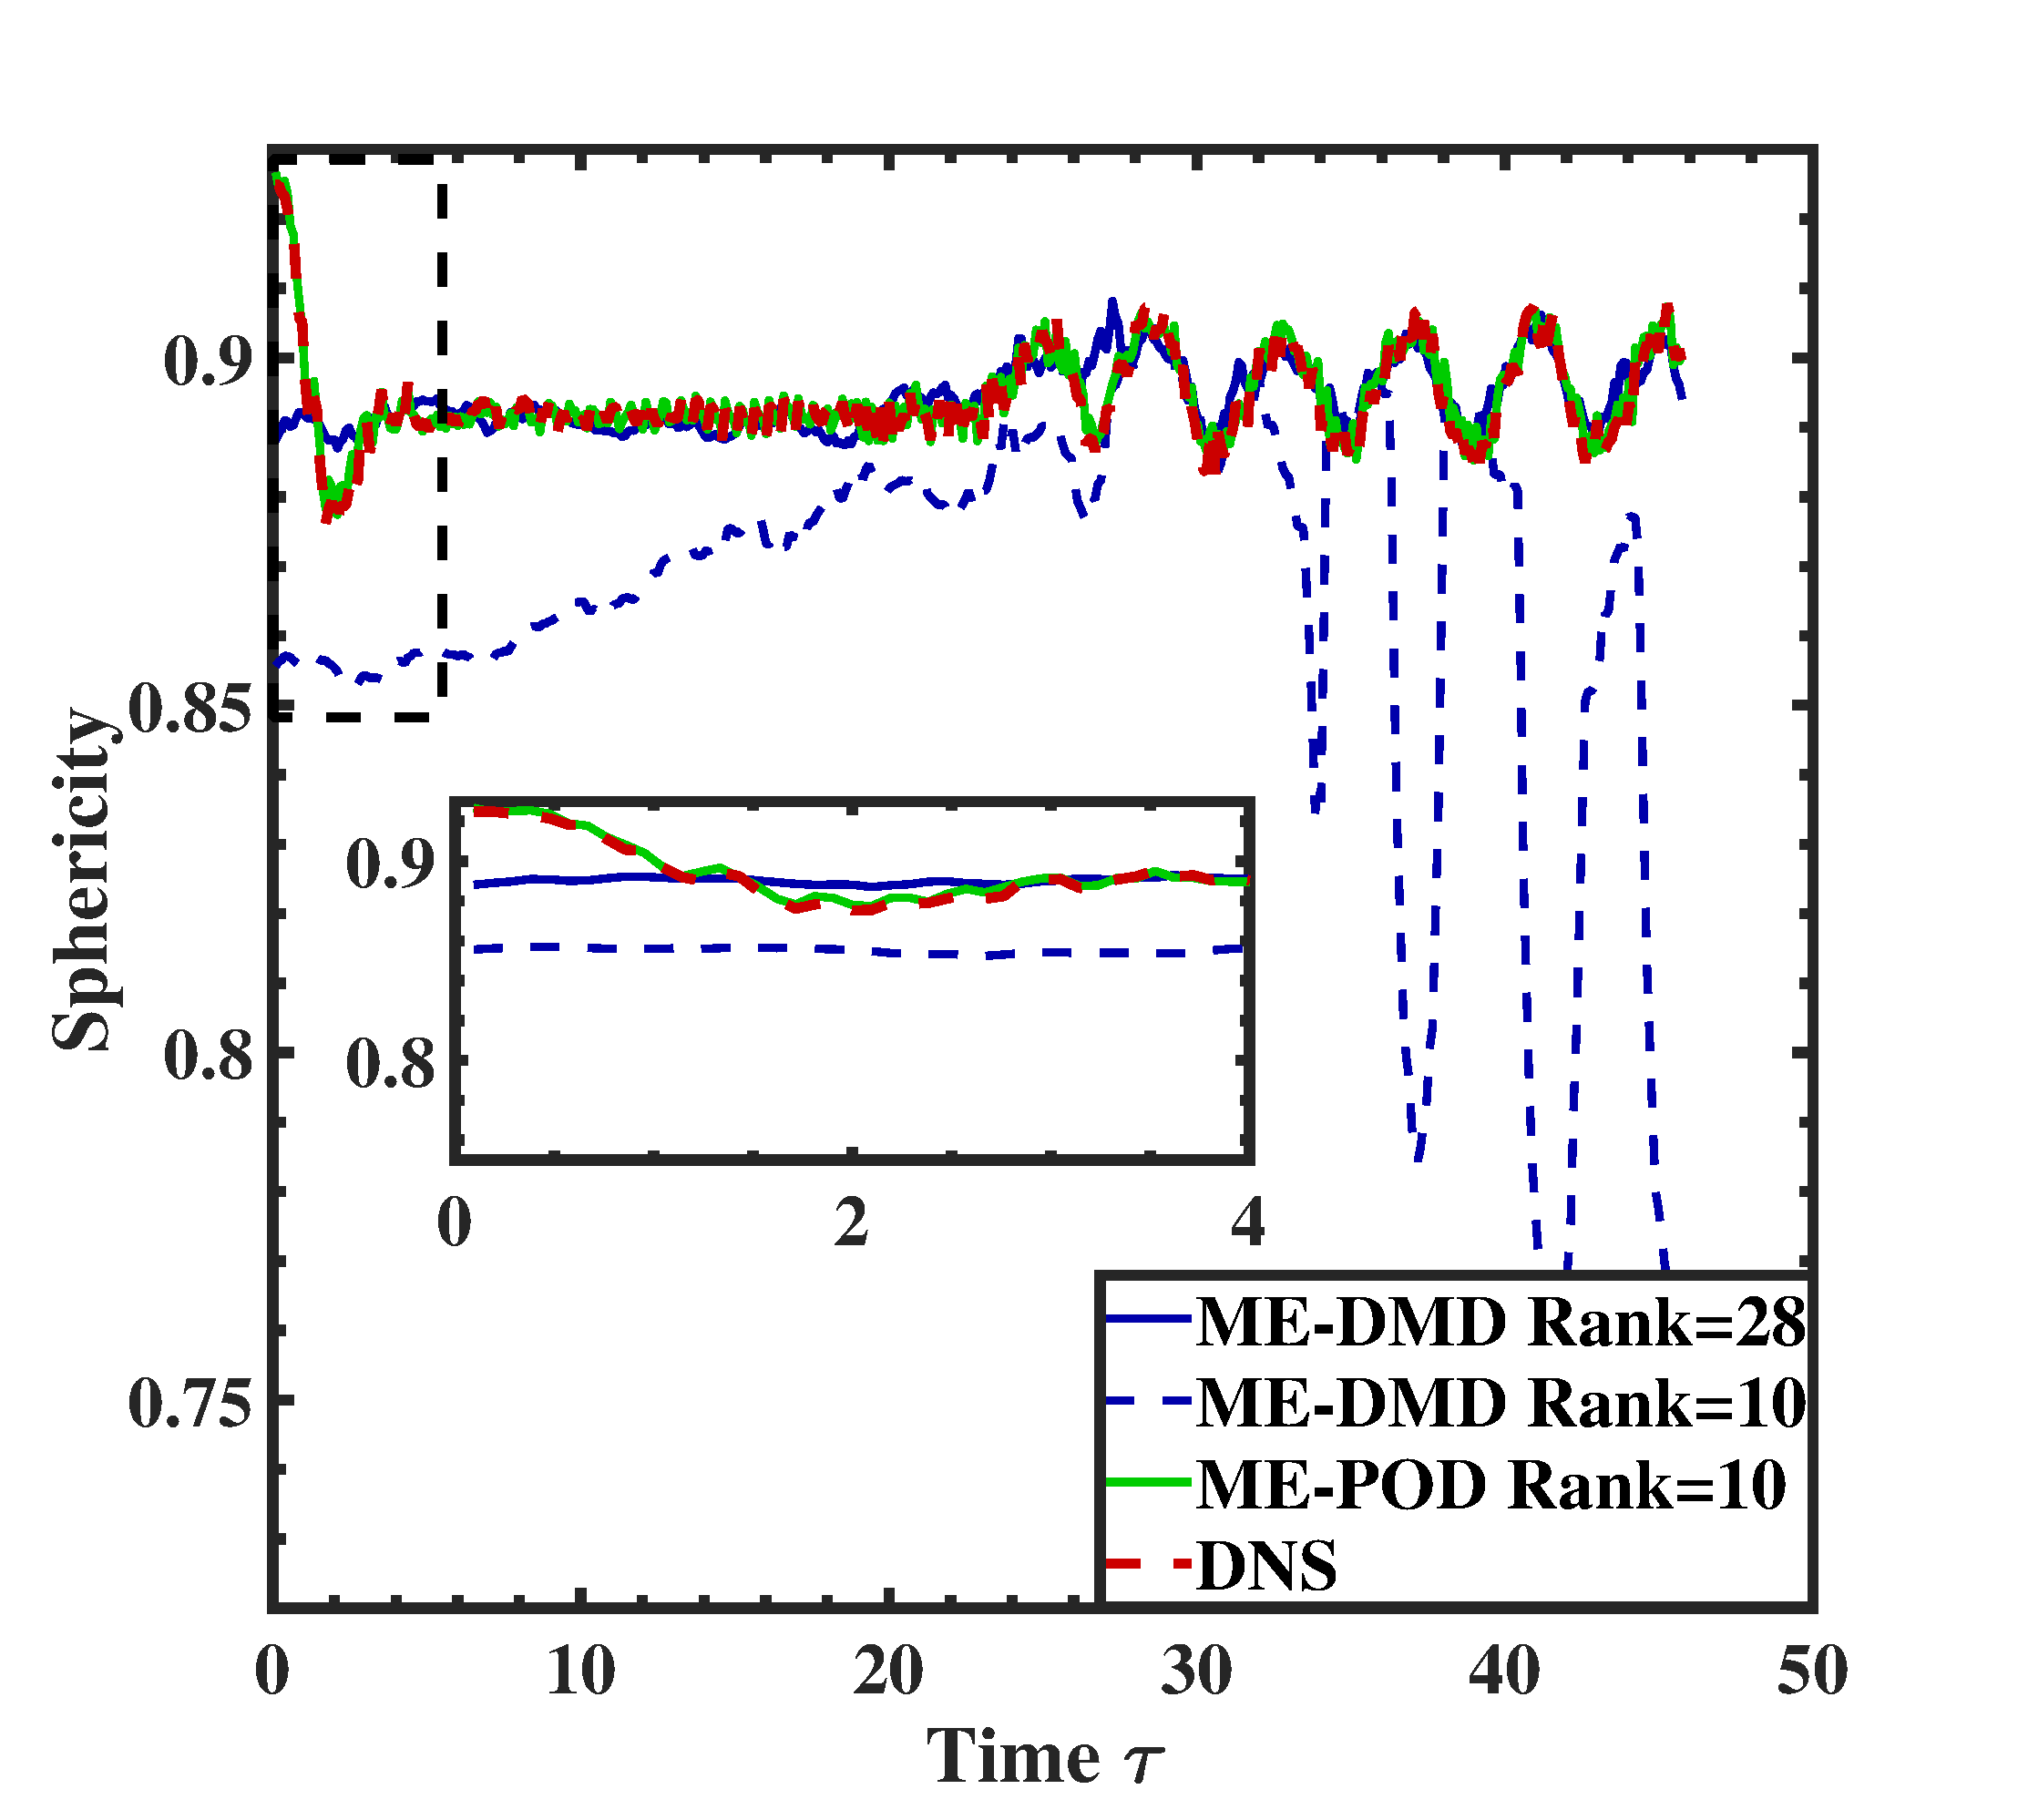
\includegraphics[scale=0.24,trim={0cm 0.3cm 2.5cm 2cm},clip]{Figure7b.eps}
		\put(-215,219){\large\textbf{(b)}}
	\end{subfigure}
	
	\vspace{0.1cm} % Add vertical space between rows if needed
	
	% Row 2: (c) and (d)
	\begin{subfigure}[t]{0.49\textwidth}
		\centering
		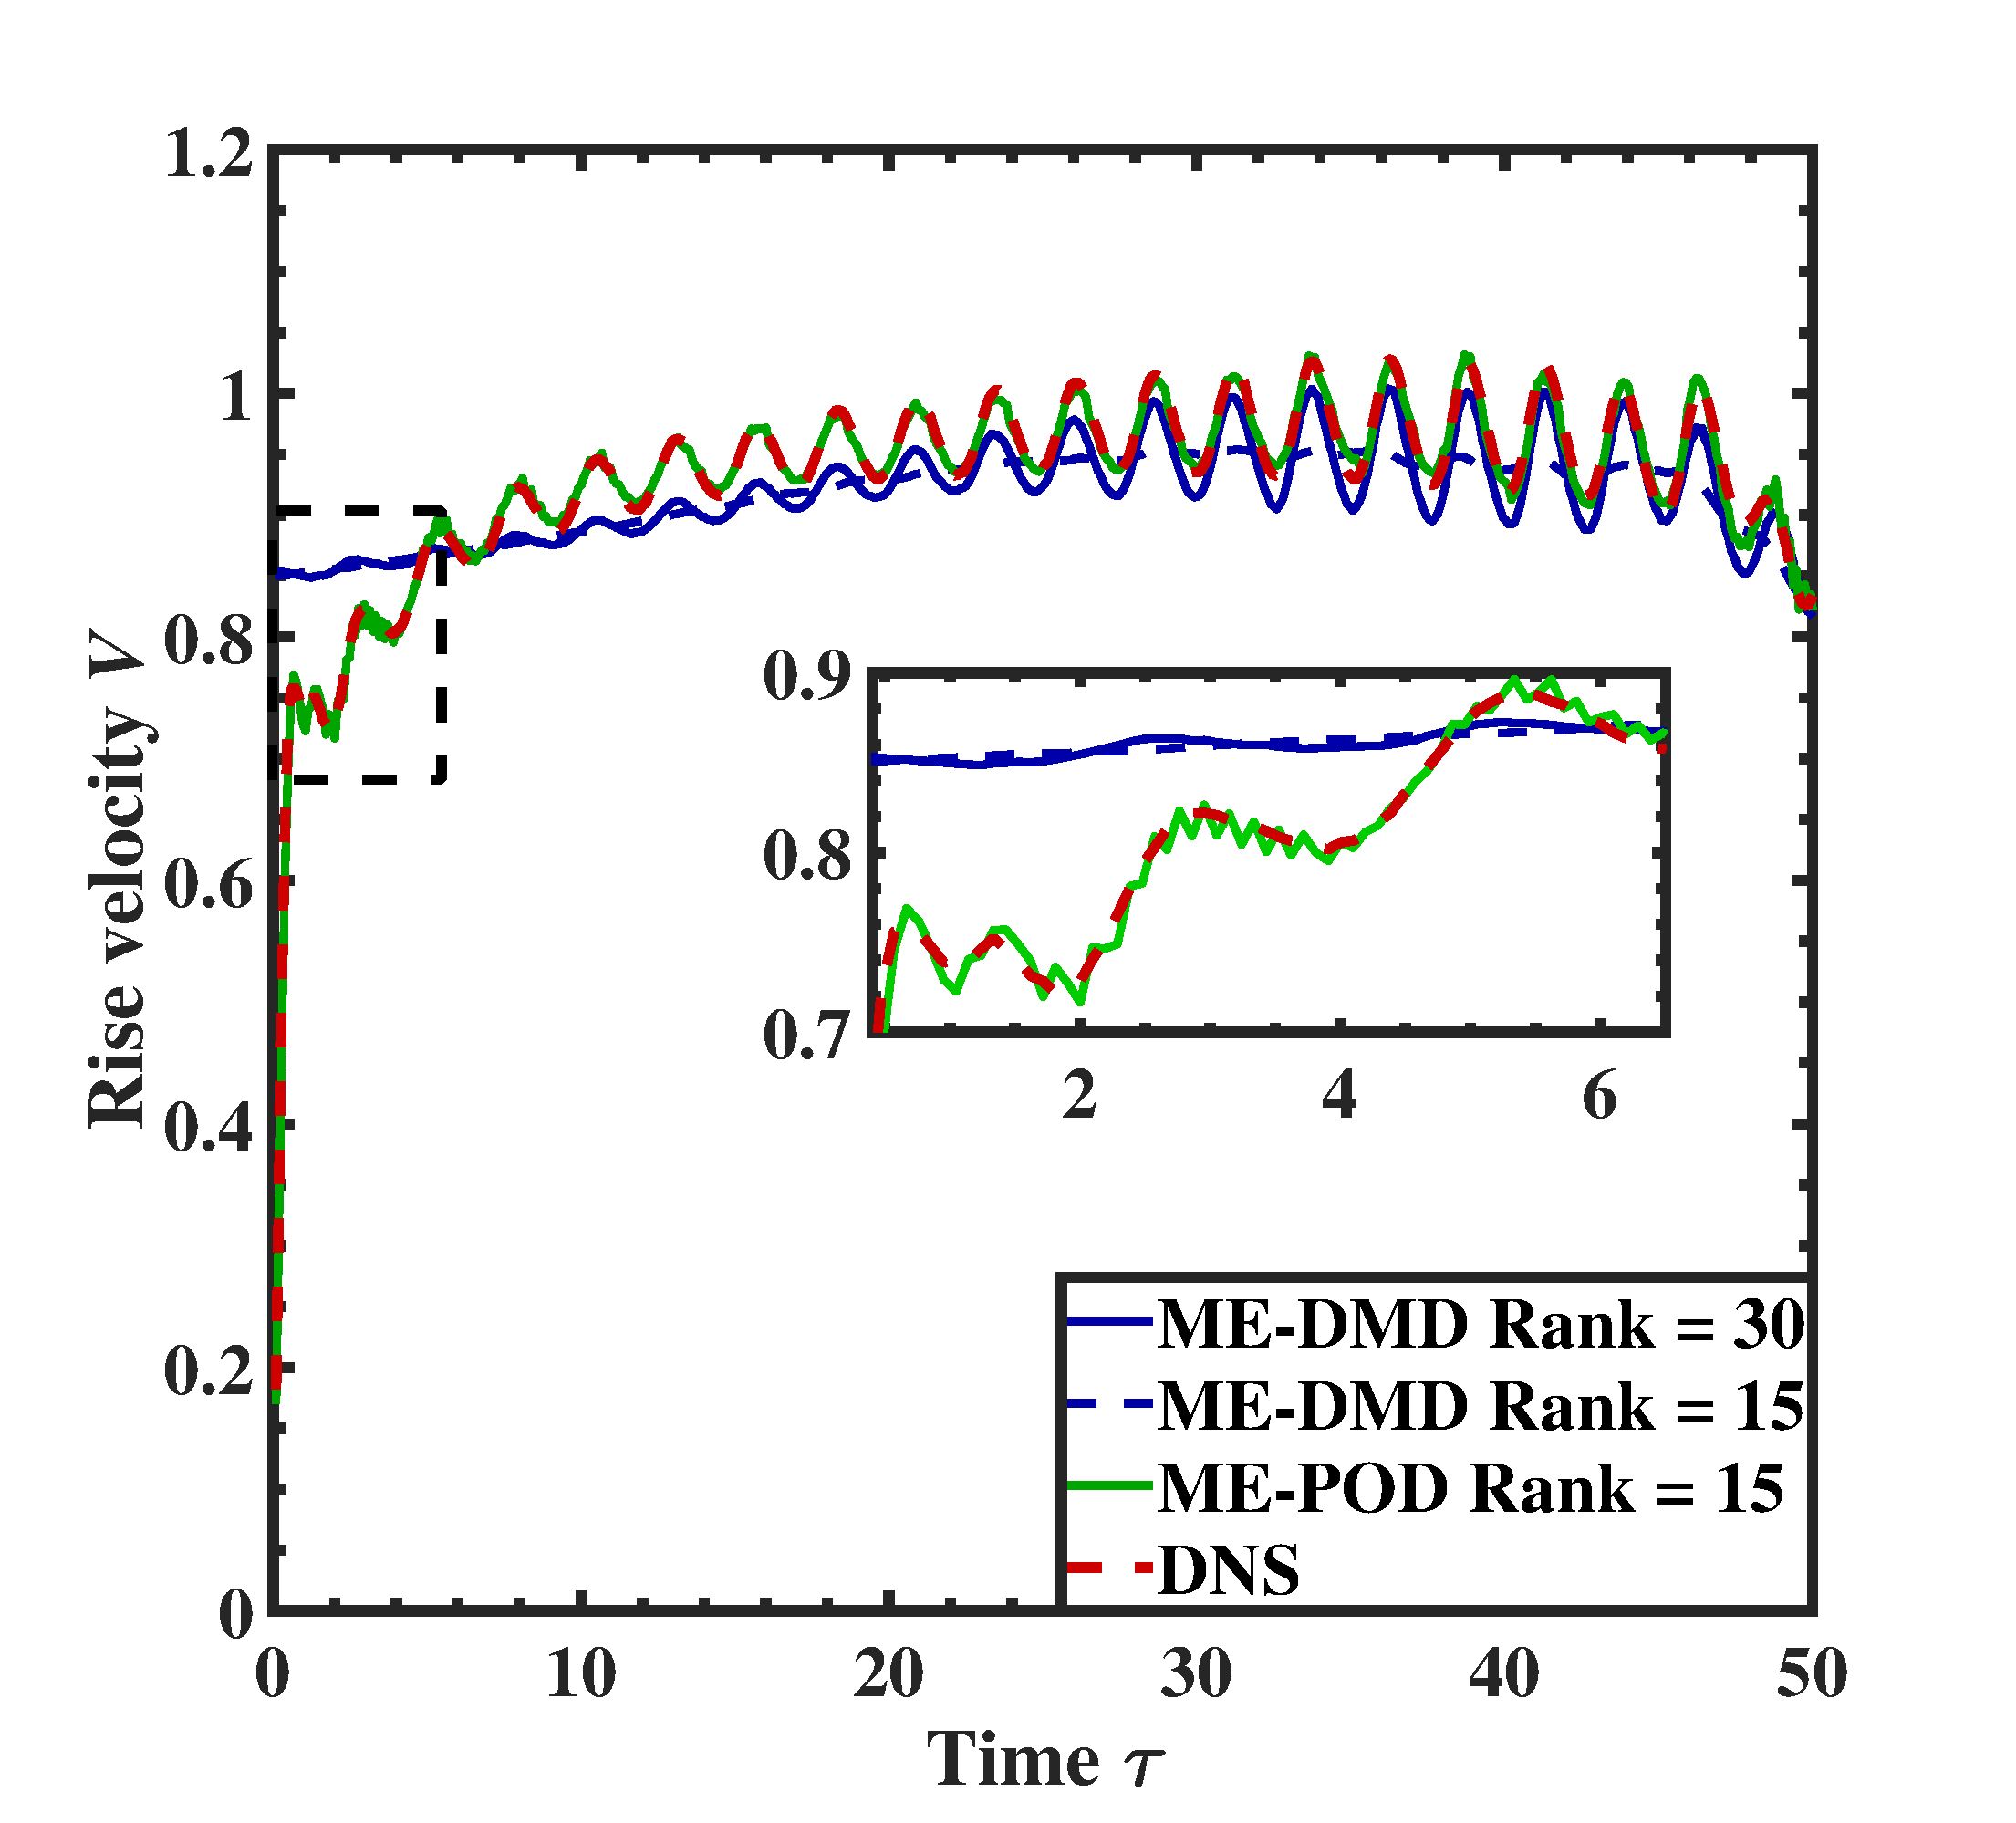
\includegraphics[scale=0.24,trim={0.5cm 0.3cm 2.5cm 2cm},clip]{Figure7c.eps}
		\put(-215,219){\large\textbf{(c)}}
	\end{subfigure}
	\hfill
	\begin{subfigure}[t]{0.49\textwidth}
		\centering
		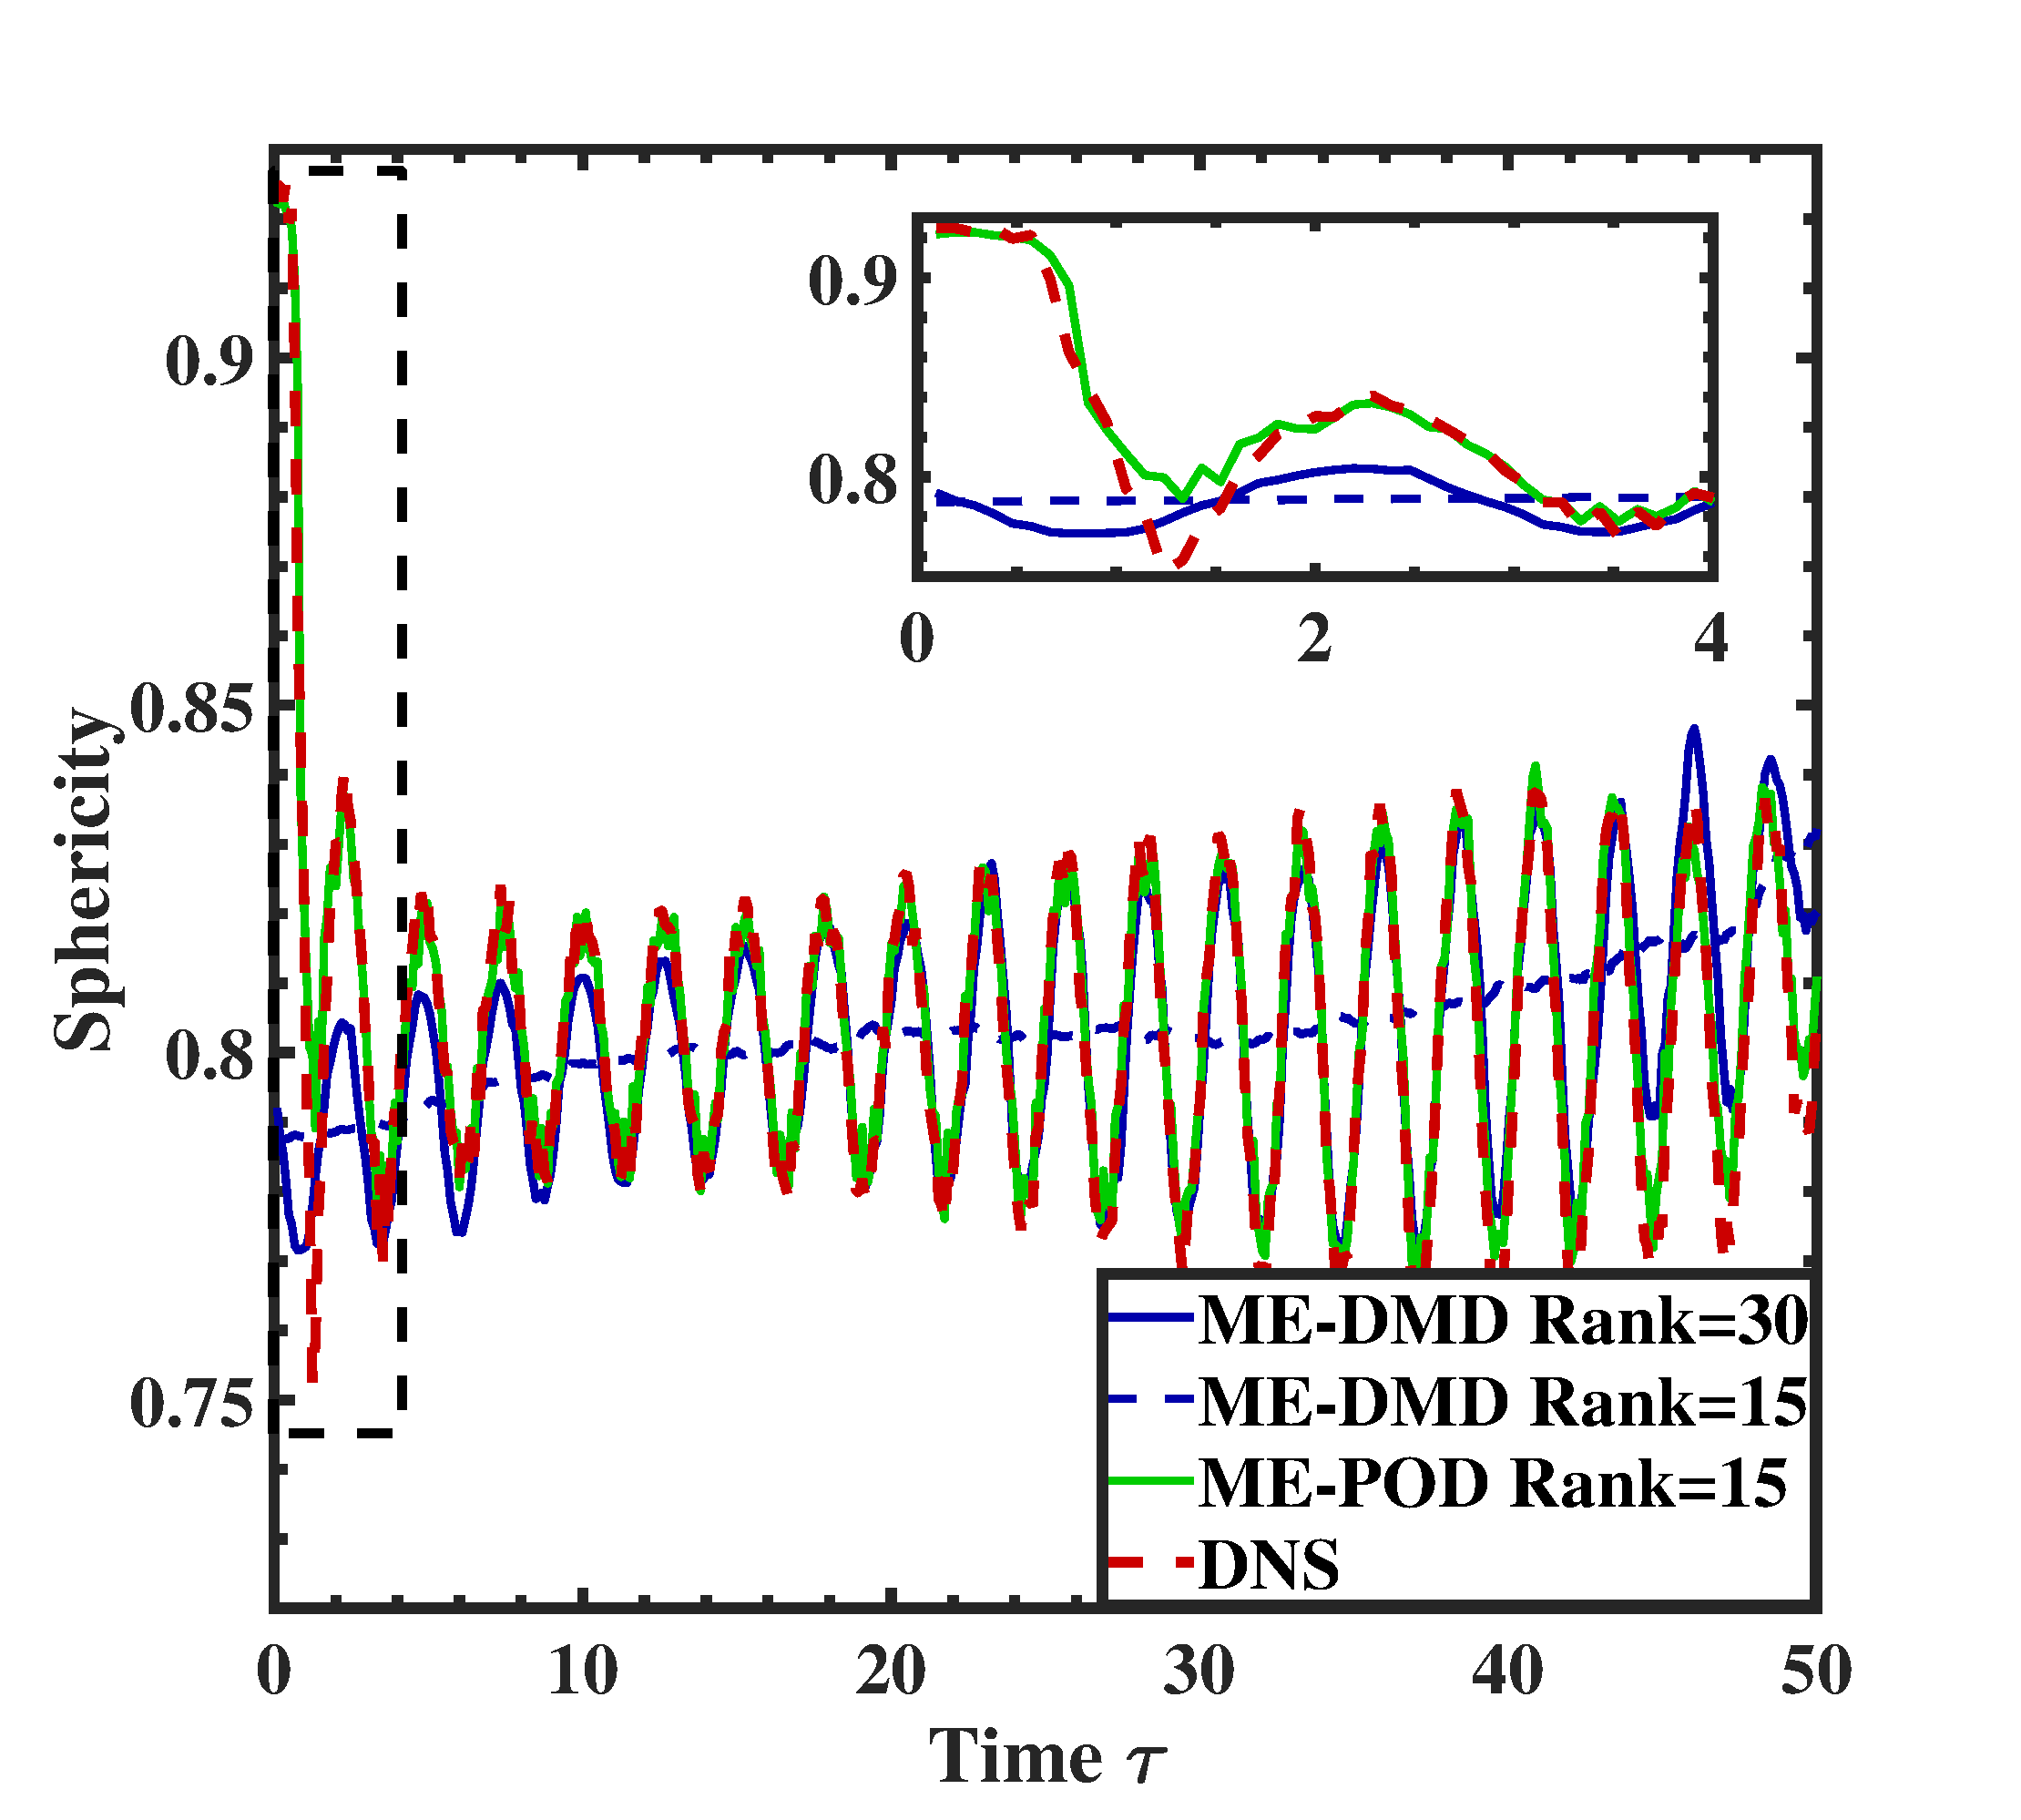
\includegraphics[scale=0.24,trim={0cm 0.3cm 2.5cm 2cm},clip]{Figure7d.eps}
		\put(-215,219){\large\textbf{(d)}}
	\end{subfigure}
	
	\caption{Rise velocity (Left) and circularity (Right) for the 3D bubble cases (a-b) C$_4$ and (c-d) C$_5$ using ME-POD and ME-DMD. The same number of modes is used for the velocity and gas volume fraction fields.}
	\label{Fig7}
\end{figure}

\end{document}